\documentclass[journal]{IEEEtran}
\usepackage[T1]{fontenc}
\usepackage{cite}
\usepackage{amsmath,amssymb,amsfonts}
\usepackage{graphicx}
\usepackage{textcomp}
\usepackage{booktabs}
\usepackage{multirow}
\usepackage{array}
\usepackage{tikz}
\usetikzlibrary{arrows.meta}
\usepackage{url}
\hyphenation{op-tical net-works semi-conduc-tor IEEE-Xplore}

\begin{document}

\title{Unified ML Pipelines: A Reproducible Study of Training-Serving Skew, Lineage, and Release Gating}

\author{Bhavin~Kotak%
\thanks{B. Kotak is with IBM, Armonk, NY, USA (e-mail: bhavin.kotak@ibm.com). ORCID: 0009-0006-4793-7046.}%
\thanks{This is version 2.0 of a preprint first released in January 2026. Version 1 reported outcome figures that no data supported; this version replaces them with a preregistered experiment that anyone can rerun.}%
}

\markboth{Preprint, version 2.0}%
{Kotak: Unified ML Pipelines: Training-Serving Skew, Lineage, and Release Gating}

\maketitle

\begin{abstract}
Machine learning systems often compute features twice, once in a batch job for training and again in a per-request service for serving. Any divergence between the two programs causes training-serving skew. Version 1 of this paper argued for unified pipelines built on a single feature definition, but no releasable data stood behind its outcome figures. This version withdraws those figures and measures the central technical claim. We formalise the two feature paths, the skew and disagreement measures, a content-hash lineage record, and a fail-closed release gate. The experiment uses three public OpenML tables with five seeds. Offline, a dual implementation with five documented divergence sources matched the AUC of a single definition; online, its ROC AUC was lower by 0.086, 0.222, and 0.139. Every 95\% confidence interval excluded zero, and the preregistered hypothesis was supported. Categorical encoding order caused most of the loss. The request-level skew rate was above 0.96 for every source, the harmless ones included, which makes it a weak proxy for harm. Prediction disagreement tracked harm more closely. The single definition stayed skew-free only while online-store lookups succeeded. Pinned reruns were bit-identical in 15 of 15 cases. When a rerun differed, only a lineage record with resolved seeds and parameters explained it. In a simulated release gate, adding an offline-online replay check raised the share of harmful candidates blocked from 0.522 to 0.970. It also blocked 53 of 98 harmless candidates. Code, data, and results are released so the study can be rerun.
\end{abstract}

\begin{IEEEkeywords}
MLOps, training-serving skew, feature store, point-in-time correctness, data lineage, reproducibility, continuous integration, software engineering for machine learning
\end{IEEEkeywords}

\IEEEpeerreviewmaketitle

\section{Introduction}
\label{sec:intro}

\IEEEPARstart{A}{} machine learning (ML) model is trained on features computed by one program and is served with features computed by another. The training features usually come from a batch job over a historical table; the serving features come from an online service that answers each request under a latency budget. If the two programs disagree, the model sees inputs at serving time that differ from the ones it was trained and validated on. This failure is called training-serving skew \cite{polyzotis2018lifecycle,breck2017mltestscore}. Production ML platforms such as TFX added shared transformation components partly to prevent it \cite{baylor2017tfx}. In interview and case studies of ML deployment, data and pipeline management keep coming up as sources of friction \cite{amershi2019se4ml,paleyes2022challenges,shankar2022interview,lwakatare2020largescale}.

Two engineering patterns are commonly proposed in response. One is a \emph{single feature definition}: the same feature logic runs for offline backfill and for online serving, typically through a feature store \cite{orr2021featurestores,feast}. The other is a unified release process. Feature code, model code, parameters, and deployment configuration are versioned together, and a change is promoted only through automated checks \cite{kreuzberger2023mlops,opengitops}. Both patterns are widely recommended. Few studies measure their effect in a way that others can rerun.

Version 1 of this paper described such an architecture and reported large organisational gains, for example shorter model-to-production time and fewer skew incidents. There was no data behind those figures that could be released or checked, so this version removes them. The architecture and the patterns stay. We state them formally and measure the central technical claim with a preregistered experiment on public data.

We ask five research questions.
\begin{itemize}[\IEEEsetlabelwidth{RQ5:}]
\item[RQ1:] Does a single feature definition give higher online discrimination (ROC AUC) than a dual implementation that contains documented, realistic divergences?
\item[RQ2:] Which divergence sources cause the harm, and is the request-level skew rate a usable proxy for that harm?
\item[RQ3:] Where does the single-definition pattern itself break (store timeouts, heavier missingness, covariate shift)?
\item[RQ4:] What must a lineage record contain so that a rerun is either bit-identical or has its difference explained?
\item[RQ5:] Does a release gate with a skew replay check block injected regressions that an accuracy-only gate promotes?
\end{itemize}

The paper makes four contributions. The first is a formal system model of the two feature paths, the skew and disagreement measures, a content-hash lineage record, and a fail-closed release gate. It comes with a reference architecture that states how every external decision point behaves under missing data, unknown results, and timeouts (Section~\ref{sec:method}). The second is an open experiment harness on three OpenML tables with five seeds, with a per-source ablation, three breakpoint scenarios, a rerun study, and a simulated gate (Section~\ref{sec:eval}). Third, we give measured answers to RQ1 to RQ5, negative and mixed results included. Fourth, we list the version 1 claims that were removed or reframed (Section~\ref{sec:threats}).

\section{Related Work}
\label{sec:related}

\subsection{Software engineering for ML}
Amershi et al.\ describe a nine-stage ML workflow at a large software company and the data-management challenges that distinguish it from conventional software \cite{amershi2019se4ml}. Paleyes et al.\ survey published deployment case studies and organise the challenges by workflow stage \cite{paleyes2022challenges}, and Lwakatare et al.\ review industrial ML systems and their challenges \cite{lwakatare2020largescale}. In interviews by Shankar et al., practitioners report that data and pipeline issues dominate operational work \cite{shankar2022interview}. Kreuzberger et al.\ define MLOps and its components from literature and interviews \cite{kreuzberger2023mlops}. These works motivate our questions. None of them measures skew under controlled conditions.

\subsection{Platforms and feature stores}
TFX puts data validation, transformation, training, and serving in one platform \cite{baylor2017tfx}. Orr et al.\ discuss feature stores as the system that manages feature definitions for both training and serving \cite{orr2021featurestores}. Feast is an open-source feature store with offline and online stores \cite{feast}. Xin et al.\ analyse a large corpus of production pipelines and their redundant computation \cite{xin2021production}. We do not evaluate any of these systems. What we implement is the pattern they share, one definition executed in both contexts, and we compare it with a dual implementation.

\subsection{Data validation and testing}
The ML Test Score lists tests for production readiness, among them checks that training and serving features agree \cite{breck2017mltestscore}. Polyzotis et al.\ survey data lifecycle challenges, training-serving skew among them \cite{polyzotis2018lifecycle}. Schelter et al.\ automate data quality verification with declarative constraints \cite{schelter2018dataquality}, and Zhang et al.\ survey ML testing \cite{zhang2022mltesting}. For continuous integration of models, Renggli et al.\ give statistically grounded conditions \cite{renggli2019easemlci}. Kaufman et al.\ formalise leakage; point-in-time violations in aggregate features are one instance of it \cite{kaufman2012leakage}. Gama et al.\ survey drift and shift detection, and Rabanser et al.\ study them empirically \cite{gama2014drift,rabanser2019failing}. Our gate combines an accuracy check of the kind studied in \cite{renggli2019easemlci} with a direct offline-online replay. We measure what each of the two catches.

\subsection{Provenance and reproducibility}
Simmhan et al.\ survey data provenance and classify systems by what they record and how \cite{simmhan2005provenance}. Vamsa infers provenance from data science scripts \cite{namaki2020vamsa}. Schlegel and Sattler survey ML artefact management \cite{schlegel2022artifacts}. Reproducibility gaps in ML research are documented by Gundersen and Kjensmo and by Pineau et al.\ \cite{gundersen2018reproducibility,pineau2020reproducibility}. Pham et al.\ measure the variance that nondeterminism adds to deep learning training \cite{pham2020variance}. Our lineage study is narrower. It asks which fields a content-hash record must include so that a rerun of a tabular model is either bit-identical or flagged.

\section{Methodology}
\label{sec:method}

\subsection{System model}
\label{sec:model}

A stream of events $r_t=(x_t,g_t,y_t)$, $t=1,\dots,N$, arrives in time order. Here $x_t$ holds numeric attributes $x_t^{\mathrm{num}}$ and categorical attributes $x_t^{\mathrm{cat}}$, $g_t$ is an entity key (one categorical attribute), and $y_t\in\{0,1\}$ is a label revealed after the prediction for $t$ is made. The history before $t$ is $H_{<t}=\{r_s : s<t\}$. Indices $t\le n$ form the training window; indices $t>n$ form the serving window $T$. A feature definition is a map $\phi(x_t,H_{<t})\in\mathbb{R}^d$. It returns imputed numeric attributes, one derived ratio $x^{(a)}/(x^{(b)}+1)$, an integer code for each categorical attribute, and three entity aggregates. Let $\mathbf{1}[\cdot]$ be the indicator function, $v_s$ the numeric attribute being aggregated, $m_v$ its training median, $\pi$ the training positive rate, and $\alpha>0$ a smoothing pseudo-count. The point-in-time aggregates for entity $g=g_t$ are
\begin{equation}
\begin{aligned}
c_g(t) &= \textstyle\sum_{s<t}\mathbf{1}[g_s=g],\\
\bar v_g(t) &= \frac{\sum_{s<t}\mathbf{1}[g_s=g]\,v_s+\alpha m_v}{c_g(t)+\alpha},\\
\rho_g(t) &= \frac{\sum_{s<t}\mathbf{1}[g_s=g]\,y_s+\alpha\pi}{c_g(t)+\alpha}.
\end{aligned}
\label{eq:pit}
\end{equation}
The sums in \eqref{eq:pit} range over $s<t$ only. That is the point-in-time constraint: a feature for event $t$ may not depend on event $t$ or on any later event \cite{kaufman2012leakage}. For an entity with no history, $c_g(t)=0$ and the aggregates equal their priors $m_v$ and $\pi$.

\subsection{Two feature paths}
\label{sec:paths}

Every system computes an offline feature vector $\phi^{\mathrm{off}}(t)$ for training and offline validation, and an online feature vector $\phi^{\mathrm{on}}(t)$ for serving. The \emph{single-definition path} executes the same function in both contexts. Offline backfill replays history through $\phi$, and serving calls $\phi$ against an online store that holds the running sums of \eqref{eq:pit}. The \emph{dual path} is two programs: a vectorised batch job $\phi^{B}_{\theta}$ for training, and a per-request function $\phi^{S}_{\theta}$, written independently, for serving. The vector $\theta\in\{0,1\}^5$ switches five divergence sources on or off:
\begin{equation}
\left(\phi^{\mathrm{off}},\phi^{\mathrm{on}}\right)=
\begin{cases}
(\phi,\ \phi) & \text{single definition},\\
(\phi^{B}_{\theta},\ \phi^{S}_{\theta}) & \text{dual implementation}.
\end{cases}
\label{eq:paths}
\end{equation}
Table~\ref{tab:sources} defines the sources of \eqref{eq:paths}. Each one mirrors a class of divergence discussed in prior work and in version 1 of this paper: imputation defaults, numeric precision in serialisation, categorical vocabulary order, aggregate freshness, and point-in-time leakage \cite{polyzotis2018lifecycle,breck2017mltestscore,kaufman2012leakage}. With $\theta=\mathbf{0}$ the dual code must reproduce $\phi$ exactly. We test this as a correctness control.

\begin{table}[!t]
\caption{Divergence Sources of the Dual Implementation}
\label{tab:sources}
\centering
\footnotesize
\setlength{\tabcolsep}{3pt}
\begin{tabular}{@{}>{\raggedright\arraybackslash}p{1.45cm}>{\raggedright\arraybackslash}p{3.3cm}>{\raggedright\arraybackslash}p{3.3cm}@{}}
\toprule
Source & Batch (training) & Per request (serving) \\
\midrule
missing default & missing numeric field $\to$ training median & missing numeric field $\to 0$ \\\addlinespace[3pt]
precision & float64, no rounding & float32 inputs; ratio and aggregates rounded to 2 decimals \\\addlinespace[3pt]
encoding order & sorted vocabulary; unknown $\to -1$ & vocabulary in first-seen file order; unknown $\to 0$ \\\addlinespace[3pt]
stale window & aggregates up to $t-1$ & aggregates from a snapshot refreshed every 1000 requests \\\addlinespace[3pt]
PIT leakage & aggregates over the whole table, including $t$ and later rows & aggregates up to $t-1$ \\
\bottomrule
\end{tabular}
\end{table}

\subsection{Measures and objective}
\label{sec:measures}

For a request $t\in T$ and feature $j$, a mismatch is recorded when the two paths differ by more than a tolerance $\epsilon=10^{-9}$ in absolute and relative terms. The request-level skew rate $S$ counts requests with at least one mismatched feature:
\begin{equation}
\begin{aligned}
m_{tj}&=\mathbf{1}\!\left[\,|\phi^{\mathrm{off}}_j(t)-\phi^{\mathrm{on}}_j(t)|>\epsilon\,(1+|\phi^{\mathrm{off}}_j(t)|)\,\right],\\
S&=\frac{1}{|T|}\sum_{t\in T}\max_{j}m_{tj}.
\end{aligned}
\label{eq:skew}
\end{equation}
We also report the cell mismatch rate $\frac{1}{|T|d}\sum_{t,j}m_{tj}$. A mismatch does harm only if it changes a decision. For a fitted scorer $f$ and threshold $\tau=0.5$, the prediction disagreement rate is
\begin{equation}
D=\frac{1}{|T|}\sum_{t\in T}\mathbf{1}\!\left[\mathbf{1}[f(\phi^{\mathrm{off}}(t))\ge\tau]\neq\mathbf{1}[f(\phi^{\mathrm{on}}(t))\ge\tau]\right].
\label{eq:disagree}
\end{equation}
Let $f_1$ be trained on $\{\phi(t)\}_{t\le n}$ and $f_2$ on $\{\phi^{B}_{\theta}(t)\}_{t\le n}$. The primary endpoint is the paired difference in online ROC AUC on the serving window,
\begin{equation}
\Delta=\mathrm{AUC}\!\left(\{f_1(\phi(t)),y_t\}_{t\in T}\right)-\mathrm{AUC}\!\left(\{f_2(\phi^{S}_{\theta}(t)),y_t\}_{t\in T}\right).
\label{eq:delta}
\end{equation}
A positive $\Delta$ means the single definition serves a better ranking than the dual implementation. The offline-online gap of a path is its offline AUC minus its online AUC. We stated the preregistered decision rule (Section~\ref{sec:setup}) on $\Delta$. $S$ is only a proxy, and the rule does not use it.

\subsection{Lineage record}
\label{sec:lineage}

Let $H(\cdot)$ be SHA-256 over a canonical serialisation. For a training run with feature matrix $F$, labels $y$, code $C$ (feature definition and model constructor source), parameters $P$, and environment $E$ (library versions), the lineage identifier is
\begin{equation}
\ell=H\!\left(H_{\mathrm{data}}(F,y)\,\|\,H(C)\,\|\,H(P)\,\|\,H(E)\right).
\label{eq:lineage}
\end{equation}
We compare two ways of filling in this record. The \emph{explicit} record hashes the data as an unordered set of rows, and hashes $P$ as the user-written parameter file, in which an unset seed is stored as \texttt{None}. The \emph{resolved} record hashes the rows in training order and stores library versions plus every constructor parameter after resolution, the concrete seed included. A rerun is bit-identical when the SHA-256 of its held-out predicted probabilities equals that of the reference run. A non-identical rerun counts as \emph{explained} if its $\ell$ differs from the reference.

\subsection{Release gate}
\label{sec:gate}

A candidate pipeline is promoted only if three checks pass on a validation window $V\subset T$ (the first half of the serving window). Let $L$ be true when every lineage field is present, $A_c$ and $A_0$ the offline AUC of the candidate and the incumbent on $V$, $\delta=0.005$ the AUC margin, $S_c$ the candidate's skew rate \eqref{eq:skew} from replaying $V$ through its offline and online paths, and $s_{\max}=0.01$ the skew limit:
\begin{equation}
\mathrm{promote}=L\wedge\left(A_c\ge A_0-\delta\right)\wedge\left(S_c\le s_{\max}\right).
\label{eq:gate}
\end{equation}
A conjunct is false when its check raises an error, times out, or returns an undefined value, such as an AUC on a single-class window. The gate therefore fails closed. The \emph{AUC-only} gate is the same rule without the last conjunct. We label a candidate \emph{harmful} if its online AUC on the post-gate window $T\setminus V$ is more than 0.005 below the incumbent's.

\subsection{Reference architecture and outcome handling}
\label{sec:arch}

Fig.~\ref{fig:arch} shows the architecture kept from version 1, cut down to the parts the experiment exercises. Feature definitions, model code, and deployment manifests live in one Git repository. The same definition feeds an offline backfill and an online store. Every training run writes the lineage record \eqref{eq:lineage}. The gate \eqref{eq:gate} decides promotion to a model registry, and a GitOps controller reconciles serving with the registry \cite{opengitops}. Table~\ref{tab:outcomes} states how each external decision point behaves when data are missing, a result is unknown, or a call times out. The released code implements these rules. Its unit tests also exercise the rules for the store, the feature definition, the gate, and the registry.

\begin{figure}[!t]
\centering
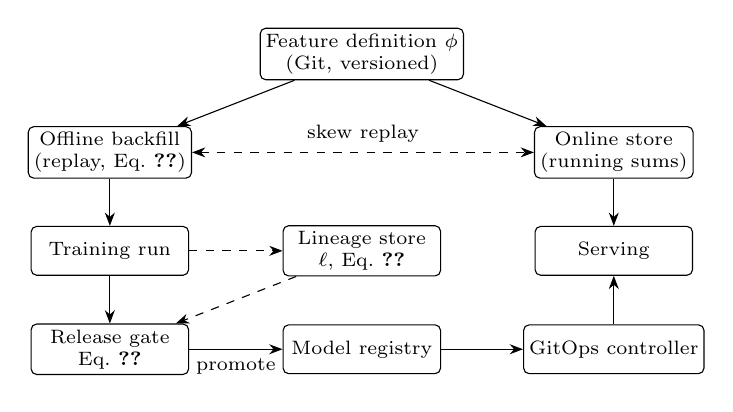
\begin{tikzpicture}[font=\scriptsize, >=Stealth,
  box/.style={draw, rounded corners=2pt, align=center, minimum height=0.62cm, minimum width=2.0cm, inner sep=2pt}]
\node[box] (def) at (4.2cm,3.75cm) {Feature definition $\phi$\\(Git, versioned)};
\node[box] (off) at (1.0cm,2.5cm) {Offline backfill\\(replay, Eq.~\ref{eq:pit})};
\node[box] (on) at (7.4cm,2.5cm) {Online store\\(running sums)};
\node[box] (train) at (1.0cm,1.25cm) {Training run};
\node[box] (lin) at (4.2cm,1.25cm) {Lineage store\\$\ell$, Eq.~\ref{eq:lineage}};
\node[box] (serve) at (7.4cm,1.25cm) {Serving};
\node[box] (gate) at (1.0cm,0cm) {Release gate\\Eq.~\ref{eq:gate}};
\node[box] (reg) at (4.2cm,0cm) {Model registry};
\node[box] (ops) at (7.4cm,0cm) {GitOps controller};
\draw[->] (def) -- (off);
\draw[->] (def) -- (on);
\draw[->] (off) -- (train);
\draw[->] (on) -- (serve);
\draw[->] (train) -- (gate);
\draw[->] (gate) -- node[below]{promote} (reg);
\draw[->] (reg) -- (ops);
\draw[->] (ops) -- (serve);
\draw[->, dashed] (train) -- (lin);
\draw[->, dashed] (lin) -- (gate);
\draw[<->, dashed] (off) -- node[above]{skew replay} (on);
\end{tikzpicture}
\caption{Reference architecture. One feature definition feeds both offline backfill and online serving. Dashed arrows carry lineage and the offline-online replay that the release gate uses. Labels refer to Eqs.~\eqref{eq:pit}, \eqref{eq:lineage}, and \eqref{eq:gate}.}
\label{fig:arch}
\end{figure}

\begin{table*}[!t]
\caption{Behaviour of External Decision Points Under Missing Data, Unknown Results, and Timeouts}
\label{tab:outcomes}
\centering
\footnotesize
\setlength{\tabcolsep}{4pt}
\begin{tabular}{@{}>{\raggedright\arraybackslash}p{2.7cm}>{\raggedright\arraybackslash}p{4.6cm}>{\raggedright\arraybackslash}p{4.6cm}>{\raggedright\arraybackslash}p{4.6cm}@{}}
\toprule
Decision point & Missing data & Unknown result & Timeout \\
\midrule
Online store lookup & Unknown entity: count 0, aggregates equal priors $m_v,\pi$ & Not applicable (lookup returns a tuple or fails) & Serve fallback (count 0, priors); mark request degraded; count in $S$ \\\addlinespace[3pt]
Feature definition & Missing numeric: training median; missing or unseen category: code $-1$ & Not applicable (pure function) & Not applicable (in process) \\\addlinespace[3pt]
Release gate check & Missing lineage field: block & Error, NaN, or single-class AUC: block (fail closed) & Treated as unknown: block \\\addlinespace[3pt]
Model registry & Requested version absent: keep incumbent & Artefact hash differs from lineage: refuse to load, keep incumbent & Keep incumbent; retry on next reconcile \\\addlinespace[3pt]
Data download (OpenML) & Not applicable (cached file used) & sha256 differs from manifest: abort run & Retry with alternate parser, then abort with error \\
\bottomrule
\end{tabular}
\end{table*}

\section{Evaluation}
\label{sec:eval}

\subsection{Setup}
\label{sec:setup}

\subsubsection{Data}
Table~\ref{tab:datasets} lists three public tables retrieved from OpenML \cite{vanschoren2014openml}: Adult \cite{uciadult}, Bank Marketing \cite{moro2014bank}, and German Credit (credit-g) \cite{ucigerman}. We drop the Bank Marketing call-duration column, since its value is known only after the outcome. Each file is cached with its SHA-256 checksum, and a mismatch aborts the run (Table~\ref{tab:outcomes}). The entity keys are occupation (Adult), job (Bank Marketing), and purpose (credit-g), and the aggregated numeric attributes are hours per week, account balance, and credit amount, in the same order. The smoothing pseudo-count in \eqref{eq:pit} is $\alpha=20$.

\begin{table}[!t]
\caption{Datasets and Serving Windows (Seed 0)}
\label{tab:datasets}
\centering
\footnotesize
\setlength{\tabcolsep}{3.5pt}
%BEGIN:tab_datasets
\begin{tabular}{@{}lrrrrrr@{}}
\toprule
Dataset & Rows & Num. & Cat. & Pos. rate & Train & Requests \\
\midrule
adult & 48842 & 6 & 8 & 0.239 & 34189 & 14653 \\
bank-marketing & 45211 & 6 & 9 & 0.117 & 31647 & 13564 \\
credit-g & 1000 & 7 & 13 & 0.300 & 700 & 300 \\
\bottomrule
\end{tabular}
%END:tab_datasets
\end{table}

\subsubsection{Event stream}
The tables carry no timestamps, so time is simulated. For each seed we draw a random arrival order. The first 70\% of arrivals form the training window, and the last 30\% are replayed one by one as serving requests. Each label is revealed as soon as its request has been scored. To exercise imputation, we inject missing-completely-at-random values into 5\% of numeric cells of every table (a simulation). Adult's own missing categories are left in place.

\subsubsection{Model}
All paths use scikit-learn's histogram gradient boosting classifier \cite{pedregosa2011sklearn} with 150 iterations, learning rate 0.1, feature subsampling 0.8, and no early stopping. Categorical codes go in as ordinal numeric inputs. Each model fit uses one OpenMP thread.

\subsubsection{Protocol}
Each dataset is run with five seeds (0 to 4). A seed fixes the arrival order, the injected missingness, and the model seed. For every dataset and seed we run the single path, the dual path with all five sources, the dual control with no source, five single-source ablations, and the single path with online-store timeout probability 0.01, 0.05, and 0.2. On a timeout the store serves the fallback of Table~\ref{tab:outcomes}. Two further breakpoint scenarios rerun the single and dual paths. In the first, missingness rises to 20\% of numeric cells, four times the base rate. The second is covariate shift: arrivals are ordered by age plus Gaussian noise whose standard deviation is 0.5 times that of age, so the serving window holds older people.

\subsubsection{Statistics and preregistration}
We report means and standard deviations over the five seeds. Paired differences get two-sided 95\% $t$ confidence intervals (4 degrees of freedom). Before the full run we registered the hypothesis, the endpoint $\Delta$ of \eqref{eq:delta}, and the rule (file \texttt{preregistration.json}): the hypothesis is SUPPORTED if, in at least two of three datasets, the mean $\Delta\ge 0.005$ and the lower confidence bound exceeds 0; REFUTED if, in at least two of three datasets, the upper bound is below 0.005; and INCONCLUSIVE otherwise. The code computes the verdict from the result files.

\subsubsection{Reproducibility study}
On the seed-0 split of each dataset, we retrain the single-path model five times under each of five regimes. They are: pinned (fixed seed, data, parameters); pinned with one versus two OpenMP threads; unpinned seed (fresh operating-system entropy, with the parameter file recording no seed); training rows in a different order with the seed pinned; and a simulated library default change (L2 regularisation 0 versus 1, not recorded in the parameter file). Each regime has its own reference run.

\subsubsection{Gate simulation}
For each dataset and seed, the incumbent is the pipeline with all sources off, and eleven candidates go through \eqref{eq:gate}. Three of them are benign: a new model seed (seed plus 1000), learning rate 0.09, and shuffled training rows. The other eight are injected regressions (simulations): 20\% of training labels flipped; one column dropped upstream (Adult capital gain, Bank Marketing previous outcome, credit-g checking status); an underfit model with 5 iterations; point-in-time leakage in the training batch job; and a serving-only bug for each of the other four sources.

\subsection{Results}
\label{sec:results}

\subsubsection{Correctness control}
With every source switched off, the dual code reproduced the single definition exactly. The maximum absolute feature difference was 0 for all three datasets and five seeds, in both the training and the serving window (file \texttt{controls.csv}). Every difference reported below is therefore caused by the switched sources.

\begin{table}[!t]
\caption{Primary Endpoint: Offline and Online ROC AUC (Mean $\pm$ SD Over Five Seeds) and Paired $\Delta$ With 95\% CI}
\label{tab:main}
\centering
\footnotesize
\setlength{\tabcolsep}{3pt}
%BEGIN:tab_main
\begin{tabular}{@{}llccc@{}}
\toprule
Dataset & Path & Offline AUC & Online AUC & Gap \\
\midrule
adult & single & 0.922$\pm$0.002 & 0.922$\pm$0.002 & 0.000 \\
 & dual & 0.924$\pm$0.002 & 0.836$\pm$0.019 & 0.088 \\
 & $\Delta$ & \multicolumn{3}{c}{0.086 [0.063, 0.109]} \\
\midrule
bank-marketing & single & 0.783$\pm$0.005 & 0.783$\pm$0.005 & 0.000 \\
 & dual & 0.794$\pm$0.003 & 0.560$\pm$0.040 & 0.234 \\
 & $\Delta$ & \multicolumn{3}{c}{0.222 [0.171, 0.274]} \\
\midrule
credit-g & single & 0.763$\pm$0.032 & 0.763$\pm$0.032 & 0.000 \\
 & dual & 0.775$\pm$0.013 & 0.625$\pm$0.071 & 0.150 \\
 & $\Delta$ & \multicolumn{3}{c}{0.139 [0.072, 0.205]} \\
\bottomrule
\end{tabular}
%END:tab_main
\end{table}

\subsubsection{Online discrimination (RQ1)}
Table~\ref{tab:main} and Fig.~\ref{fig:auc} give the primary endpoint. On offline validation the two paths look alike; on Adult the dual path scored 0.924 and the single path 0.922. Online, the dual path fell to 0.836, 0.560, and 0.625 on Adult, Bank Marketing, and credit-g, while the single path served exactly its offline AUC. The paired difference $\Delta$ of \eqref{eq:delta} was 0.086 [0.063, 0.109] on Adult, 0.222 [0.171, 0.274] on Bank Marketing, and 0.139 [0.072, 0.205] on credit-g. All three datasets met the preregistered support condition, so the verdict computed by the code is SUPPORTED. For the dual path, the offline-online gap was 0.088, 0.234, and 0.150, respectively. Offline validation alone did not reveal it.

\begin{figure}[!t]
\centering
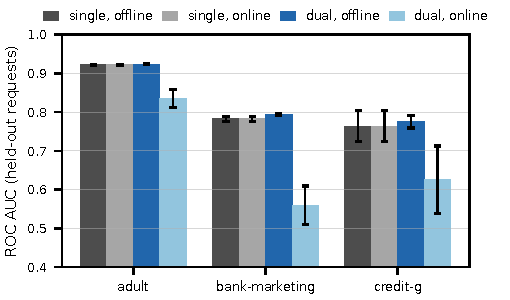
\includegraphics[width=\columnwidth]{figures/fig_auc.pdf}
\caption{Offline and online ROC AUC on the serving window for the single definition and the dual implementation with all five sources (mean over five seeds; error bars show 95\% CI half-widths).}
\label{fig:auc}
\end{figure}

\begin{figure*}[!t]
\centering
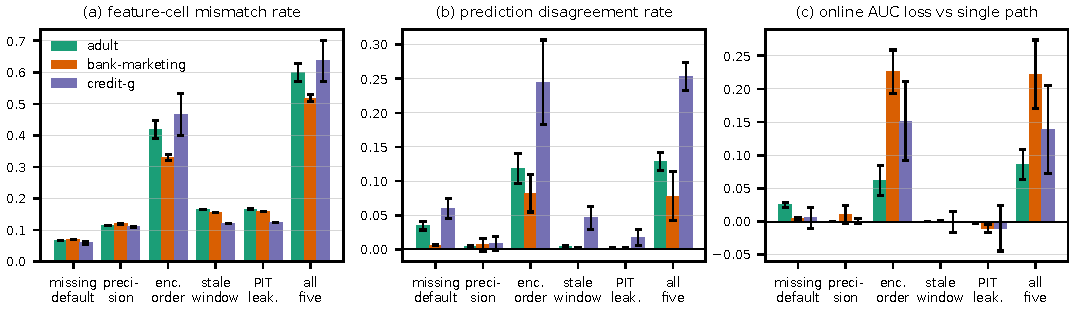
\includegraphics[width=\textwidth]{figures/fig_ablation.pdf}
\caption{Single-source ablation of the dual implementation. (a) Fraction of feature cells that differ between offline and online paths. (b) Fraction of requests whose thresholded prediction flips. (c) Online AUC loss relative to the single path, $\Delta$ of \eqref{eq:delta}. Means over five seeds; error bars are 95\% CI half-widths.}
\label{fig:ablation}
\end{figure*}

\begin{table}[!t]
\caption{Single-Source Ablation (Means Over Five Seeds). Req.\ Skew Is $S$ of \eqref{eq:skew}; Disagree Is $D$ of \eqref{eq:disagree}}
\label{tab:ablation}
\centering
\footnotesize
\setlength{\tabcolsep}{2.4pt}
%BEGIN:tab_ablation
\begin{tabular}{@{}llrrrr@{}}
\toprule
Dataset & Source & Req. skew & Cell mism. & Disagree & $\Delta$AUC \\
\midrule
adult & missing default & 1.000 & 0.067 & 0.034 & 0.025 \\
 & precision & 1.000 & 0.115 & 0.004 & 0.000 \\
 & encoding order & 1.000 & 0.418 & 0.119 & 0.062 \\
 & stale window & 0.985 & 0.164 & 0.003 & 0.000 \\
 & PIT leakage & 1.000 & 0.167 & 0.002 & -0.002 \\
 & all five & 1.000 & 0.599 & 0.129 & 0.086 \\
\midrule
bank-marketing & missing default & 1.000 & 0.071 & 0.006 & 0.004 \\
 & precision & 1.000 & 0.120 & 0.007 & 0.011 \\
 & encoding order & 1.000 & 0.330 & 0.082 & 0.226 \\
 & stale window & 0.988 & 0.156 & 0.001 & 0.000 \\
 & PIT leakage & 1.000 & 0.158 & 0.002 & -0.011 \\
 & all five & 1.000 & 0.518 & 0.078 & 0.222 \\
\midrule
credit-g & missing default & 0.965 & 0.059 & 0.059 & 0.006 \\
 & precision & 0.999 & 0.110 & 0.009 & 0.001 \\
 & encoding order & 1.000 & 0.466 & 0.245 & 0.151 \\
 & stale window & 0.967 & 0.121 & 0.046 & -0.001 \\
 & PIT leakage & 1.000 & 0.125 & 0.017 & -0.010 \\
 & all five & 1.000 & 0.636 & 0.253 & 0.139 \\
\bottomrule
\end{tabular}
%END:tab_ablation
\end{table}

\subsubsection{Which sources cause harm (RQ2)}
Table~\ref{tab:ablation} and Fig.~\ref{fig:ablation} attribute the effect to sources. Categorical encoding order alone produced most of it, with $\Delta$ of 0.062 on Adult, 0.226 on Bank Marketing, and 0.151 on credit-g. On Adult the second source was the missing-value default, at 0.025 [0.022, 0.029]. On Bank Marketing that source gave 0.004 [0.002, 0.006], and on credit-g its interval included 0. Precision rounding and the stale window changed online AUC by at most 0.011 in absolute value, and all of their intervals included 0. Point-in-time leakage gave a negative $\Delta$ on Adult ($-0.002$) and Bank Marketing ($-0.011$), so the leaky model served slightly better rankings. Our entity keys have between 10 and 14 values. Each whole-table aggregate therefore averages thousands of rows, and the leaked label carries little weight. Leakage through high-cardinality keys, the case discussed in \cite{kaufman2012leakage}, was not tested.

The request-level skew rate did not separate harmful from harmless sources. Every source produced $S\ge 0.96$, the harmless ones too, because once any input to an aggregate feature differs, that feature differs on almost every request. With all sources on, all 73265 Adult requests (five seeds) were skewed, while 9438 of them (0.129) changed their thresholded prediction. The prediction disagreement rate $D$ tracked harm more closely. On every dataset the two sources with the largest $D$ were also the two with the largest $\Delta$, and encoding order ranked first on both. The cell mismatch rate did not track harm: point-in-time leakage touched 0.167 of Adult feature cells, more than the missing default (0.067), and still caused no loss. A skew monitor that alarms on $S$ alone would alarm on every source. One that alarms on $D$ would do so roughly in proportion to harm.

\begin{figure}[!t]
\centering
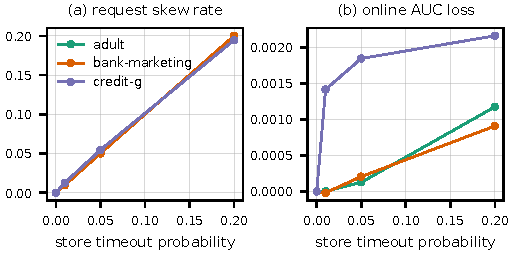
\includegraphics[width=\columnwidth]{figures/fig_timeout.pdf}
\caption{Single definition with online-store timeouts. A timeout serves the documented fallback (priors). (a) Request skew rate. (b) Online AUC loss relative to the same path without timeouts. Means over five seeds.}
\label{fig:timeout}
\end{figure}

\begin{table}[!t]
\caption{Breakpoint Scenarios: Online AUC (Mean Over Five Seeds) and Paired $\Delta$ With 95\% CI}
\label{tab:breakpoints}
\centering
\footnotesize
\setlength{\tabcolsep}{2.5pt}
%BEGIN:tab_breakpoints
\begin{tabular}{@{}llccc@{}}
\toprule
Dataset & Scenario & Single & Dual & $\Delta$ [95\% CI] \\
\midrule
adult & base & 0.922 & 0.836 & 0.086 [0.063, 0.109] \\
 & 4x missing & 0.914 & 0.748 & 0.166 [0.128, 0.204] \\
 & shift & 0.886 & 0.823 & 0.063 [0.054, 0.073] \\
\midrule
bank-marketing & base & 0.783 & 0.560 & 0.222 [0.171, 0.274] \\
 & 4x missing & 0.781 & 0.541 & 0.240 [0.189, 0.291] \\
 & shift & 0.784 & 0.549 & 0.235 [0.195, 0.276] \\
\midrule
credit-g & base & 0.763 & 0.625 & 0.139 [0.072, 0.205] \\
 & 4x missing & 0.753 & 0.612 & 0.141 [0.095, 0.188] \\
 & shift & 0.748 & 0.628 & 0.120 [0.011, 0.229] \\
\bottomrule
\end{tabular}
%END:tab_breakpoints
\end{table}

\subsubsection{Where the single definition breaks (RQ3)}
The single definition is free of skew only as long as every store lookup succeeds. In Fig.~\ref{fig:timeout} the skew rate tracked the timeout probability: on Adult it was 0.0097, 0.0504, and 0.1995 for timeout probabilities 0.01, 0.05, and 0.2. Every degraded request was skewed and no other request was (14619 of 73265 Adult requests at probability 0.2). The degraded flag of Table~\ref{tab:outcomes} thus identifies skewed requests exactly. The harm was small, because the fallback replaces only the three aggregates. At probability 0.2 the online AUC loss was 0.0012 [0.0004, 0.0020] on Adult, and the intervals for Bank Marketing and credit-g included 0.

Table~\ref{tab:breakpoints} covers the other two breakpoints. Raising missingness to 20\% of numeric cells nearly doubled $\Delta$ on Adult, from 0.086 to 0.166 [0.128, 0.204], because the zero fill of the serving path now fires four times as often. The single path's online AUC was 0.914 here, against 0.922 at the base rate. Under covariate shift by age, $\Delta$ stayed positive on all three datasets: 0.063 [0.054, 0.073], 0.235 [0.195, 0.276], and 0.120 [0.011, 0.229].

\begin{table}[!t]
\caption{Rerun Study (Three Datasets, Five Reruns Each). Identical: Bit-Identical Held-Out Predictions. Expl.: Non-Identical Reruns Whose Lineage Hash \eqref{eq:lineage} Changed}
\label{tab:repro}
\centering
\footnotesize
\setlength{\tabcolsep}{3pt}
%BEGIN:tab_repro
\begin{tabular}{@{}lrrrr@{}}
\toprule
Regime & Identical & Differ & Expl. (explicit) & Expl. (resolved) \\
\midrule
pinned & 15/15 & 0 & 0/0 & 0/0 \\
pinned, 1 vs 2 threads & 15/15 & 0 & 0/0 & 0/0 \\
unpinned seed & 0/15 & 15 & 0/15 & 15/15 \\
row order varies & 15/15 & 0 & 0/0 & 0/0 \\
default change (sim.) & 6/15 & 9 & 0/9 & 9/9 \\
\bottomrule
\end{tabular}
%END:tab_repro
\end{table}

\subsubsection{What lineage must record (RQ4)}
Table~\ref{tab:repro} summarises the five regimes. With seed, data, and parameters pinned, all 15 reruns produced bit-identical held-out predictions, and so did the reruns that alternated between one and two OpenMP threads. With the seed left unset, none of the 15 reruns matched its reference, and predicted probabilities moved by up to 0.465. The explicit record stores the seed as unset. It changed in none of these 15 cases and so could not explain the difference, while the resolved record, which stores the concrete seed, changed in all 15. The simulated library default change behaved the same way: 9 of 15 reruns differed, the explicit record explained none of them, and the resolved record explained all 9. Reordering the training rows changed no prediction of this learner. Even so, the order-sensitive data hash of the resolved record flagged all 15 such reruns. An order-sensitive hash is thus conservative. It never missed a real change in our runs, but it raised false alarms for an order-invariant learner.

\begin{table}[!t]
\caption{Simulated Release Gate: Harmful Candidates and Candidates Blocked per Gate, Over 15 Dataset-Seed Pairs. Skew Rate Is the Mean $S_c$ on the Validation Window}
\label{tab:gate}
\centering
\footnotesize
\setlength{\tabcolsep}{2.5pt}
%BEGIN:tab_gate
\begin{tabular}{@{}lrrrr@{}}
\toprule
Candidate & Harmful & AUC-only & AUC+skew & Skew rate \\
\midrule
seed change & 0/15 & 2/15 & 2/15 & 0.000 \\
learning rate 0.09 & 0/15 & 2/15 & 2/15 & 0.000 \\
row shuffle & 0/15 & 0/15 & 0/15 & 0.000 \\
\midrule
label noise & 14/15 & 15/15 & 15/15 & 0.000 \\
dropped column & 13/15 & 13/15 & 13/15 & 0.000 \\
underfit & 9/15 & 11/15 & 11/15 & 0.000 \\
training PIT leakage & 1/15 & 2/15 & 15/15 & 1.000 \\
serving encoding order & 15/15 & 0/15 & 15/15 & 1.000 \\
serving missing default & 10/15 & 0/15 & 15/15 & 0.988 \\
serving stale window & 1/15 & 0/15 & 15/15 & 0.969 \\
serving precision & 4/15 & 0/15 & 15/15 & 1.000 \\
\bottomrule
\end{tabular}
%END:tab_gate
\end{table}

\subsubsection{What the release gate catches (RQ5)}
Table~\ref{tab:gate} lists every candidate. All regressions in it are injected simulations. Of 165 candidate evaluations, 67 were harmful by the post-gate criterion. The AUC-only gate blocked 35 of them (0.522), and the gate with the skew replay of \eqref{eq:gate} blocked 65 (0.970). The difference came from two kinds of change that do not lower offline AUC. Serving-only bugs do not touch the offline path, so the AUC-only gate promoted every one of them, all 15 encoding-order bugs included, though each of those was harmful. Point-in-time leakage raised offline AUC, and the AUC-only gate blocked only 2 of 15 leaky candidates. The skew replay blocked all of these.

The skew replay cost precision. The full gate blocked 53 of 98 harmless candidates (0.541), against 10 (0.102) for the AUC-only gate, because it blocked every precision and stale-window candidate when only 4 and 1 of 15 were harmful. Both gates blocked the same 4 of 45 benign changes, all on credit-g. Its validation window has 150 requests, and there the AUC margin of 0.005 is smaller than seed-to-seed variation. The two harmful candidates that passed both gates were on Bank Marketing, a dropped column and an underfit model; their AUC drop on the validation window stayed within the margin. The skew limit $s_{\max}=0.01$ treats a harmless rounding difference the same as a harmful encoding bug. RQ2 suggests that a limit on the disagreement rate $D$ would track harm more closely, but we did not evaluate such a gate.

\section{Threats to Validity}
\label{sec:threats}

\subsection{Construct validity}
The author injected the divergence sources. Their magnitudes (for example, a fill value of 0, two-decimal rounding, a refresh every 1000 requests) were fixed in the preregistration before the full run, but other choices would give other effect sizes. Readers can recombine sources from the per-source ablation. It does not estimate how often each source occurs in practice. Version 1 reported an incident taxonomy with frequencies; those frequencies had no releasable data and are not used. The primary endpoint is ROC AUC on the serving window. We report the skew rate $S$ as a proxy, and our results show that it is a weak one.

\subsection{Internal validity}
The single path and the dual control share static constants (medians, vocabularies, priors) fitted on the training window, so the paths differ only in the switched sources. The control test confirms that, with all sources off, the dual code reproduces the single definition exactly. Labels are revealed with zero delay. In a real system with delayed labels, the label-rate aggregate would be staler for both paths. Before the preregistered full run, the code was developed with unit tests and smoke runs (seed 0 of Adult and all seeds of credit-g). The smoke runs exposed two defects, both fixed before the full run: OpenMP thread oversubscription, and the reference run of the unpinned-seed regime. The full run was started twice. We stopped the first attempt during the rerun study because of OpenMP stalls on a shared machine; its skew results were identical to those of the second. No dataset, seed, divergence parameter, or threshold was changed after either run.

\subsection{External validity}
Three tabular datasets with synthetic arrival orders are not production event streams. The tables have no timestamps, so time is simulated by random permutation, and the shift scenario by ordering on age. We use one model family, gradient-boosted trees with ordinal category codes; models with one-hot or embedding inputs react differently to encoding-order errors. The online store is an in-process dictionary, not Feast, Redis, or another networked store. Timeouts are therefore simulated by a Bernoulli draw, and latency is not measured. We did not test scale beyond a single process (two orders of magnitude more entities or requests per second), nor adversarial inputs. Feast, TFX Transform, and commercial feature stores were not available as baselines in this setting and are not compared.

\subsection{Reproducibility study}
We simulated library-version changes by changing one default parameter; no different library versions were installed. Thread-count variation covers one and two OpenMP threads on one machine, and other hardware may behave differently. The rerun study uses one split per dataset.

\subsection{Release gate}
Every regression in the gate study is an injected simulation. The harm label depends on a 0.005 AUC margin on a post-gate window, and for credit-g that window is small, so the credit-g gate outcomes are noisy. The gate study does not measure engineering cost or time to detection.

\subsection{Removed or reframed version 1 claims}
No releasable data supports the following statements of version 1, and they are withdrawn: reduced model-to-production time, reduced skew incidents, faster recovery, lower infrastructure cost, higher engineer productivity, the Netflix, bank, and healthcare case-study tables, an offline-to-production AUC drop in a financial deployment, an incident taxonomy with percentages, and claims of preventing most skew-related incidents. Statements that feature stores eliminate skew are reframed. In our setting the single definition produced no skew only while every store lookup succeeded.

\section{Conclusion}
\label{sec:conclusion}

Version 1 of this paper argued for unified ML pipelines with outcome figures that nobody could check. This version keeps the architecture and states it formally. It also measures the central technical claim on public data. In our preregistered experiment, a single feature definition served better rankings than a dual implementation with five documented divergence sources on all three datasets, and offline validation of the dual path did not show the loss. Most of the loss came from one source, categorical encoding order. Two sources produced near-universal feature mismatches with no measurable harm. The request-level skew rate is therefore a weak alarm signal, and prediction disagreement is a better one. Under online-store timeouts the single definition did not remove skew. It confined skew to the requests whose lookup timed out, which the degraded flag identifies, and the resulting AUC loss was small. Pinned reruns were bit-identical, and only a lineage record that stores resolved seeds and parameters explained the reruns that were not. In the simulated gate, an offline-online replay check blocked harmful serving-side and leakage candidates that an accuracy-only gate promoted, at the price of blocking many harmless candidates.

Within the limits listed in Section~\ref{sec:threats}, these results support three rules for practice. Execute one feature definition in both contexts, and test the dual-path control for exact equality. Monitor the prediction disagreement between offline and online features as well as the feature mismatches. Record resolved seeds, full parameters, and ordered data hashes in the lineage record, and fail the release gate closed when any check is unknown.

Data and code are in the Zenodo package of this version: the paper source, the experiment code, the cached OpenML files with their sources, licences, and SHA-256 checksums (\texttt{data/SOURCES.md}), all result files including \texttt{verdict.json}, the unit tests, and the preregistration. Running \texttt{python code/run\_all.py} regenerates every number, table, and figure, and \texttt{python -m pytest tests} runs the tests.

\section*{Acknowledgment}
Generative AI was used to prepare this revision. Large language models (GitHub Copilot with Anthropic Claude) critiqued the methodology, generated the experiment code, and drafted and edited the text; in a final pass the same models also edited the wording. Every reported number, table, and figure was produced by code from logged experiment results. None of them was written by a language model. The author is employed by IBM, and this work received no external funding.

\IEEEtriggeratref{13}
\bibliographystyle{IEEEtran}
\bibliography{references}

\end{document}
